\section{Time of Flight Detector (TOF)}

	Το σύστημα Time of Flight (TOF), εγκαταστάθηκε στο STAR για την ταυτοποίηση των αδρονίων που παράγονται από τις συγκρούσεις βαρέων ιόντων. Αποτελείται από δύο υπο-ανιχνευτές, τον Pseudo Vertex Position Detector (pVPD) και τον Time of Fligh Patch (TOFp). 
	Ο πρώτος πρόκειται για τον ανιχνευτή που λαμβάνει το αρχικό σήμα, από την λήψη του οποίου ξεκινά η έναρξη του χρονομέτρου. Αποτελείται από δύο ξεχωριστά μέρη που τοποθετούνται δίπλα από τις βάσεις και έξω από τον μαγνήτη του STAR.
	Το κάθε μέρος απαρτίζεται από πλαστικούς σπινθηριστές των οποίων τα παραγόμενα φωτόνια οδηγούνται σε φωτοπολλαπλασιαστές.
	%Οταν ο TOFp λάβει σήμα, τότε σταματάει η καταμέτρηση του χρόνου. Αυτός βρίσκεται ακριβώς έξω από τον TPC
	
	Ο TOFp βρίσκεται ακριβώς έξω από τον TPC και όταν λάβει σήμα σταματάει η καταμέτρηση του χρόνου. Αποτελείται από 120 σειρές που τοπθετούνται γύρω από τον TPC. Η κάθε σειρά καλύπτει $6^o$ στην αζιμουθιακή διεύθυνση, έχει μήκος 2.4m και αποτελείται από 32 Multi-gap Resistive Plate Chambers (MRPC). 
	Ο MRPC  είναι μία συστοιχία από παράλληλα επίπεδα στο ενδιάμεσο των οποίων υπάρχει ένα αέριο.
	 Το κάθε επίπεδο αποτελεί ένα ηλεκτρόδιοστο οποίο εφαρμόζεται υψηλή τάση με αποτέλεσμα την δημιουργία ισχυρού πεδίου στο εσωτερικό τους. Όταν ένα φορτισμένο σωματίδιο διέρχεται από το αέριο δημιουργεί χιονοστοιβάδες Townsend και έτσι επάγεται φορτίο στα ηλεκτρόδια το οποίο ανινχεύεται ως σήμα.
	Η συνολική χρονική διακριτική ικανότητα του συστήματος είναι 100ps, κάτι που επιτρέπει ταυτοποίηση $\pi/K/p$ με ορμές έως και $1.6GeV/c$.
	
		\begin{figure}[h!]
				\centering
				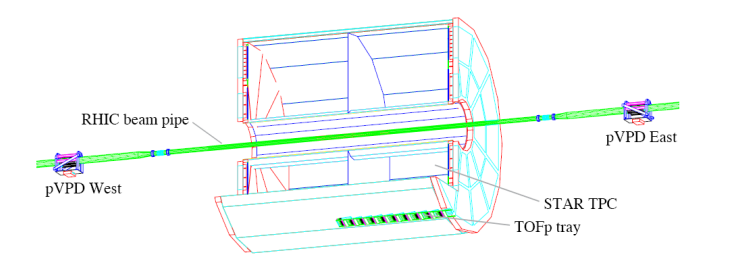
\includegraphics[scale=0.6]{STAR_Detectors/TOF}
				\caption{Οι θέσεις των υποανιχνευτών του συστήματος TOF}
				\label{fig3.27}
			\end{figure}
				
	
	Η ταυτοποίηση των σωματιδίων βασίζεται στον υπολογισμό της μάζας τους. Συγκεκριμένα, μετράται απ' ευθείας η ταχύτητα 
		\begin{align}\label{eq3.14}
			\frac{1}{\beta} = \frac{t-t_0}{\Delta s}c
		\end{align}
	όπου $\Delta s$ είναι το μήκος της τροχιάς του σωματιδίου όπως μετράται από τον TPC και $t_0$ είναι η στιγμή της κρούσης που μετράται από τον VPD. Έπειτα, η μάζα του σωματιδίου υπολογίζεται από την σχέση 
		\begin{align}\label{eq3.15}
			m = \frac{p}{c}\sqrt{\left(\frac{1}{\beta}\right)^2-1}
		\end{align}
	όπου η ορμή p μετράται από τον TPC.